% !TEX TS-program = pdflatex
% !TEX encoding = UTF-8 Unicode

% This is a simple template for a LaTeX document using the "article" class.
% See "book", "report", "letter" for other types of document.

\documentclass[11pt]{scrartcl} % use larger type; default would be 10pt

\usepackage[utf8]{inputenc} % set input encoding (not needed with XeLaTeX)

%%% Examples of Article customizations
% These packages are optional, depending whether you want the features they provide.
% See the LaTeX Companion or other references for full information.

%%% PAGE DIMENSIONS
\usepackage{geometry} % to change the page dimensions
\geometry{a4paper} % or letterpaper (US) or a5paper or....
% \geometry{margin=2in} % for example, change the margins to 2 inches all round
% \geometry{landscape} % set up the page for landscape
%   read geometry.pdf for detailed page layout information

\usepackage{graphicx} % support the \includegraphics command and options

% \usepackage[parfill]{parskip} % Activate to begin paragraphs with an empty line rather than an indent

%%% PACKAGES
\usepackage{booktabs} % for much better looking tables
\usepackage{array} % for better arrays (eg matrices) in maths
\usepackage{paralist} % very flexible & customisable lists (eg. enumerate/itemize, etc.)
\usepackage{verbatim} % adds environment for commenting out blocks of text & for better verbatim
\usepackage{subfig} % make it possible to include more than one captioned figure/table in a single float
\usepackage{graphicx}
% These packages are all incorporated in the memoir class to one degree or another...
\usepackage{hyperref}

%%% SECTION TITLE APPEARANCE
\usepackage{sectsty}
\allsectionsfont{\sffamily\mdseries\upshape} % (See the fntguide.pdf for font help)
% (This matches ConTeXt defaults)

%%% ToC (table of contents) APPEARANCE
\usepackage[nottoc,notlof,notlot]{tocbibind} % Put the bibliography in the ToC
\usepackage[titles,subfigure]{tocloft} % Alter the style of the Table of Contents
\renewcommand{\cftsecfont}{\rmfamily\mdseries\upshape}
\renewcommand{\cftsecpagefont}{\rmfamily\mdseries\upshape} % No bold!


\usepackage{amssymb}
\usepackage{amsmath}
\usepackage{mathcomp}
%\usepackage{colortbl}
\usepackage{dsfont}
\usepackage{amsfonts}
\usepackage{cancel}

%%% KV-Diagramme
%\usepackage[ngerman]{babel}
\input kvmacros

%%% Graphen
\usepackage{tikz}
\usetikzlibrary{intersections}
\usetikzlibrary{calc}

% last page
\usepackage{pageslts}

%%% END Article customizations

%%% HEADERS & FOOTERS
\usepackage{fancyhdr} % This should be set AFTER setting up the page geometry
%\usepackage{scrpage2} % Another package (only use fancyhdr or scrpage2)
\pagestyle{fancy} % options: empty , plain , fancy
\renewcommand{\headrulewidth}{1.2pt} % customise the layout...
\renewcommand{\footrulewidth}{0.1pt} % customise the layout...
\lhead{MACHINE LEARNING 1\\Andres Fernandez -- 5692442 -- fr\_andres@msn.com}\chead{}\rhead{Exercise Sheet 4 \\November 28, 2016}
\lfoot{}\cfoot{\thepage/\lastpageref{LastPages}}\rfoot{}



%%% THE SYMBOLS FOR ``DEPENDENT'' AND ``INDEPENDENT''
\newcommand{\CI}{\mathrel{\text{\scalebox{1.07}{$\perp\mkern-10mu\perp$}}}} % independent
\newcommand{\nCI}{\cancel{\mathrel{\text{\scalebox{1.07}{$\perp\mkern-10mu\perp$}}}}} % dep
%% THE SYMBOL FOR DOESN'T IMPLY
\newcommand{\notimplies}{%
  \mathrel{{\ooalign{\hidewidth$\not\phantom{=}$\hidewidth\cr$\implies$}}}}

%%% The "real" document content comes below...


\begin{document}

\section*{\\[3mm]Exercise 1}
         {\it For the one-dimensional case, show that the product of two normal distributions with means \(\mu_1, \mu_2\) and variances \(\sigma_1^2, \sigma_2^2\) is proportional to a normal distribution with mean between the original two means and variance smaller than either of the original variances.}
  

         \subsection*{i)}
         Again, the one-dimensional PDF of the normal distribution is as follows:
         \begin{equation}\label{eq:1}
           f(x|\mu,\sigma^2) =\frac{1}{\sqrt{2\pi\sigma^2}} %\mathcal{N}
           \exp\left(-\frac{1}{2}\frac{(x-\mu)^2}{\sigma^2} \right)
         \end{equation}

         \subsection*{ii)}
         With this, the product of two normal PDFs is:
         \begin{equation}\label{eq:2}
           \begin{split}
             &\frac{1}{\sqrt{2\pi\sigma_1^2}} 
           \exp\left(-\frac{1}{2}\frac{(x-\mu_1)^2}{\sigma_1^2} \right) \cdot \frac{1}{\sqrt{2\pi\sigma_2^2}} 
           \exp\left(-\frac{1}{2}\frac{(x-\mu_2)^2}{\sigma_2^2} \right)\\
           &= \frac{1}{\sqrt{2\pi\sigma_1^2}} \frac{1}{\sqrt{2\pi\sigma_2^2}}
           \exp\left(-\frac{1}{2}\frac{(x-\mu_1)^2}{\sigma_1^2} \right)  
           \exp\left(-\frac{1}{2}\frac{(x-\mu_2)^2}{\sigma_2^2} \right)\\
           &= \frac{1}{2\pi\sigma_1\sigma_2}
           \exp\left(-\frac{1}{2}\left(\frac{(x-\mu_1)^2}{\sigma_1^2}+\frac{(x-\mu_2)^2}{\sigma_2^2} \right)\right)\\
           &= \frac{1}{2\pi\sigma_1\sigma_2}
           \exp\left(-\frac{1}{2}\left(\frac{\sigma_2^2(x-\mu_1)^2}{\sigma_1^2\sigma_2^2}+\frac{\sigma_1^2(x-\mu_2)^2}{\sigma_1^2\sigma_2^2} \right)\right)\\
           &= \frac{1}{2\pi\sigma_1\sigma_2}
           \exp \left(-\frac{1}{2}\frac{\sigma_2^2(x-\mu_1)^2+\sigma_1^2(x-\mu_2)^2}{\sigma_1^2\sigma_2^2} \right)\\
           \end{split}
         \end{equation}
         \subsection*{iii)}
         Expanding the second term in the exponent (see attached paper; {\it``P. A. Bromiley: Products and Convolutions of Gaussian Probability Density Functions''}), follows:
         \begin{equation}\label{eq:2}
           \begin{split}
             &\frac{\sigma_2^2(x-\mu_1)^2+\sigma_1^2(x-\mu_2)^2}{\sigma_1^2\sigma_2^2}\\
             \text{(expand/reformulate)}&=\frac{(\sigma_1^2+\sigma_2^2)x^2 -2(\mu_1\sigma_2^2+\mu_2\sigma_1^2)x+\mu_1^2\sigma_2^2+\mu_2^2\sigma_1^2}{\sigma_1^2\sigma_2^2}\\
             \text{(div. through coeff. of }x^2)&= \frac{x^2 -2(\frac{\mu_1\sigma_2^2+\mu_2\sigma_1^2}{\sigma_1^2+\sigma_2^2})x+\frac{\mu_1^2\sigma_2^2+\mu_2^2\sigma_1^2}{\sigma_1^2+\sigma_2^2}}{\frac{\sigma_1^2\sigma_2^2}{\sigma_1^2+\sigma_2^2}}\\
             \text{(compress quad.)}&= \frac{(x - \frac{\mu_1\sigma_2^2+\mu_2\sigma_1^2}{\sigma_1^2+\sigma_2^2})^2}{\frac{\sigma_1^2\sigma_2^2}{\sigma_1^2+\sigma_2^2}}\\
           \end{split}
         \end{equation}
         Which is analogous to the expression in the exponent of the normal, one-dimensional PDF \(\frac{(x-\mu)^2}{\sigma^2}\), whereas the new values would be:
         \begin{equation}\label{eq:2}
           \begin{split}
             &\sigma_{XY} = \sqrt{\frac{\sigma_1^2\sigma_2^2}{\sigma_1^2+\sigma_2^2}}\\
             &\mu_{XY} = \frac{\mu_1\sigma_2^2+\mu_2\sigma_1^2}{\sigma_1^2+\sigma_2^2}
           \end{split}
         \end{equation}
         \subsection*{iv)}
         Now it is possible to reformulate the whole function, as well as its proportionality, with this new terms:
         \begin{equation}\label{eq:1}
           f(x,y) =\frac{1}{2\pi\sigma_1^2\sigma_2^2}
           \exp\left(-\frac{1}{2}\frac{(x-\mu_{XY})^2}{\sigma_{XY}^2} \right) \propto \exp\left(-\frac{1}{2}\frac{(x-\mu_{XY})^2}{\sigma_{XY}^2} \right)
         \end{equation}

         \subsection*{v)}
         Taking the simplified, proportional expression, it only remains to show that \(\mu_{XY}\) is between \(\mu_1\) and \(\mu_2\), and that \(\sigma_{XY}^2 < min(\sigma_1^2,\sigma_2^2)\). This can be done assuming \(\mu_1 \leq \mu_2\) (the opposite would work the same way), and \(\sigma_1^2, \sigma_2^2 \in \mathbb{R}^+\):
         \begin{equation}\label{eq:1}
           \begin{split}
             &\mu_{XY} = \frac{\mu_1\sigma_2^2+\mu_2\sigma_1^2}{\sigma_1^2+\sigma_2^2} \geq \frac{\mu_1\sigma_2^2+\mu_1\sigma_1^2}{\sigma_1^2+\sigma_2^2} = \frac{\mu_1(\sigma_1^2+\sigma_2^2)}{\sigma_1^2+\sigma_2^2} = \mu_1 \iff \mu_{XY} \geq \mu_1\\
             &\mu_{XY} = \frac{\mu_1\sigma_2^2+\mu_2\sigma_1^2}{\sigma_1^2+\sigma_2^2} \leq \frac{\mu_2\sigma_2^2+\mu_1\sigma_1^2}{\sigma_1^2+\sigma_2^2} = \frac{\mu_2(\sigma_1^2+\sigma_2^2)}{\sigma_1^2+\sigma_2^2} = \mu_2 \iff \mu_{XY} \leq \mu_2\\
             &\sigma_{XY} = \sqrt{\frac{\sigma_1^2\sigma_2^2}{\sigma_1^2+\sigma_2^2}} <
             \sqrt{\frac{\sigma_1^2\sigma_2^2}{\sigma_1^2}} = \sqrt{\sigma_2^2} = \sigma_2 \iff
             \sigma_{XY} < \sigma_2\\
             &\sigma_{XY} = \sqrt{\frac{\sigma_1^2\sigma_2^2}{\sigma_1^2+\sigma_2^2}} <
             \sqrt{\frac{\sigma_1^2\sigma_2^2}{\sigma_2^2}} = \sqrt{\sigma_1^2} = \sigma_1 \iff
             \sigma_{XY} < \sigma_1\\
           \end{split}
         \end{equation}
         \begin{flushright}
           $\square$\\
         \end{flushright}

         

\vspace{5mm}
\section*{Exercise 2}
         {\it Let \(p(x|\mu)\) be a univariate Gaussian \(\mathcal{N}(\mu, \sigma^2)\) with unknown parameter mean, which is also assumed to follow a Gaussian \(\mathcal{N}(\mu_0, \sigma_0^2)\). From the theory exposed before we have
           \begin{align*}
             p(\mu|X) = \frac{p(X|\mu)p(\mu)}{p(X)} = \frac{1}{\alpha}\prod_{k=1}^N\{p(x_k|\mu)p(\mu)\}
           \end{align*}

           Where for a given training data set X, p(X) is a constant denoted as \(\alpha\). Write down the explicit expression for \(p(\mu|X)\)}

         
         \subsection*{i)}
         Since \(p, \mu\) are assumed to be normally distributed, their PDFs can also be explicitly formulated:

         \begin{equation}\label{eq:2}
           \begin{split}
             &\mu \sim \mathcal{N}(\mu_0, \sigma_0^2) \iff p(\mu) = \frac{1}{\sqrt{2\pi\sigma_0^2}} %\mathcal{N}
             \exp\left(-\frac{1}{2}\frac{(\mu-\mu_0)^2}{\sigma_0^2} \right)\\
             &p(x_k|\mu) = \frac{1}{\sqrt{2\pi\sigma^2}} \exp\left(-\frac{1}{2}\frac{(x_k-\mu)^2}{\sigma^2} \right)
             = \frac{1}{\sqrt{2\pi\sigma^2}} \exp\left(-\frac{1}{2}\frac{(\mu-x_k)^2}{\sigma^2} \right)\\
             &p(x_k|\mu)p(\mu) = \frac{1}{2\pi\sigma_0\sigma} \exp\left(-\frac{1}{2}\left(\frac{(\mu-x_k)^2}{\sigma^2} +  \frac{(\mu-\mu_0)^2}{\sigma_0^2}\right)\right)\\
           \end{split}
         \end{equation}
         \subsection*{ii)}
         Which, as we already saw, corresponds to a function proportional to a normal PDF:
         \begin{equation}\label{eq:2}
           \begin{split}
             &\sigma_{H} = \sqrt{\frac{\sigma^2\sigma_0^2}{\sigma^2+\sigma_0^2}}\\
             &\mu_{H} = \frac{\mu\sigma_0^2+\mu_0\sigma^2}{\sigma^2+\sigma_0^2}\\
             p(x_k|\mu)p(\mu) &= \frac{1}{2\pi\sigma_0\sigma} \exp\left(-\frac{1}{2}\frac{(\mu-\mu_H)^2}{\sigma_H^2}\right)\\
           \end{split}
         \end{equation}
         \subsection*{iii)}
         The important note here is that, since both \(x\) and \(\mu\) are normally distributed, \(p(x_k|\mu)\propto p(\mu|x_k)\), because the PDF is based on the euclidean (or \(L_2\), or {\it radial}) distance between both of them, and this distance is symmetric (as it has to be in every norm). Therefore, and after re-normalizing it, \textbf{the expression can be directly reformulated as depending on} \(\boldsymbol{\mu}\), and the conditioned PDF remains as follows:
         \begin{equation}\label{eq:2}
           \begin{split}
             p(\mu|X) &= \frac{p(X|\mu)p(\mu)}{p(X)} = \frac{1}{\alpha}\prod_{k=1}^N\{p(x_k|\mu)p(\mu)\} = \frac{1}{\alpha}\prod_{k=1}^N \{\frac{1}{2\pi\sigma_0\sigma}\exp\left(-\frac{1}{2}\frac{(\mu-\mu_H)^2}{\sigma_H^2}\right)\}\\
             &= \frac{1}{\alpha(2\pi\sigma_0\sigma)^N}\exp\left(-\frac{1}{2\sigma_H^2}\sum_{k=1}^N\{(\mu-\mu_H)^2\}\right)\\
           \end{split}
         \end{equation}


         \vspace{5mm}
\section*{Exercise 3}
         {\it Show that, given a number of samples, \(N\), the posterior \(p(\mu|X)\) turns out to be also Gaussian, that is
           \begin{align*}
             p(\mu|X) = \frac{1}{\sigma_N\sqrt{2\pi}} \exp\left(-\frac{1}{2}\frac{(\mu-\mu_N)^2}{\sigma_N^2}\right)\\
           \end{align*}

           with mean value
           \begin{align*}
             \mu_{N} = \frac{N\sigma_0^2\overline{x}_N+\sigma^2\mu_0}{N\sigma_0^2+\sigma^2}\\
           \end{align*}
           and variance
           \begin{align*}
             \sigma_{N}^2 = \frac{\sigma^2\sigma_0^2}{N\sigma_0^2+\sigma^2}\\
           \end{align*}
           Where \(\overline{x}_N=\frac{1}{N}\sum_{k=1}^N x_k\). In the limit of large N, what happens to the mean value \(\mu_N\) and to the standard deviation \(\sigma_N\)?}

         
         \subsection*{i)}
         Assuming the samples aren't correlated to each other, and following the central limit theorem, the following is to be assumed:
         \begin{equation}\label{eq:2}
           \begin{split}
             &p(\mu) = \mathcal{N}(\mu|\mu_0, \sigma_0^2) = \frac{1}{\sqrt{2\pi\sigma_0^2}} \exp\left(-\frac{1}{2}\frac{(x-\mu_0)^2}{\sigma_0^2} \right)\\
             &p(X|\mu, \sigma) = \prod_{k=1}^N\{p(x_k|\mu, \sigma)\} = \prod_{k=1}^N\{\mathcal{N}(x_k|\mu, \sigma)\} = \frac{1}{(2\pi\sigma^2)^{\frac{N}{2}}}\exp\left(-\frac{1}{2\sigma^2}\sum_{k=1}^N\{(x_k-\mu)^2\}\right)\\
             &p(X) = \frac{1}{N}\\
           \end{split}
         \end{equation}
         \subsection*{ii)}
         With this setup, and assuming a known \(\sigma\), Bayes' theorem applies:
         \begin{align*}
           \begin{split}
             p(\mu|X) &= \frac{p(X|\mu)p(\mu)}{p(X)} =\\
             &= N \frac{1}{(2\pi\sigma^2)^{\frac{N}{2}}}\exp\left(-\frac{1}{2\sigma^2}\sum_{k=1}^N\{(x_k-\mu)^2\}\right) \frac{1}{\sqrt{2\pi\sigma_0^2}} \exp\left(-\frac{1}{2}\frac{(x-\mu_0)^2}{\sigma_0^2} \right)\\
             &= N \frac{1}{(2\pi)^{\frac{N}{2}}\sigma^N\sigma_0}\exp\left(-\frac{1}{2\sigma^2}\sum_{k=1}^N\{(x_k-\mu)^2\}-\frac{1}{2}\frac{(x-\mu_0)^2}{\sigma_0^2} \right)\\
             &= N \frac{1}{(2\pi)^{\frac{N}{2}}\sigma^N\sigma_0}\exp\left(-\frac{1}{2}\left(\frac{\sum_{k=1}^N\{(x_k-\mu)^2\}}{\sigma^2}+\frac{(\mu-\mu_0)^2}{\sigma_0^2}\right)\right)\\
           \end{split}
         \end{align*}
         Again, expanding the second term of the exponential function yields:
         \begin{align*}
           \begin{split}
             &\frac{\sum_{k=1}^N\{(x_k-\mu)^2\}}{\sigma^2}+\frac{(\mu-\mu_0)^2}{\sigma_0^2}= \frac{\sigma_0^2\sum_{k=1}^N\{(x_k-\mu)^2\} + \sigma^2(\mu-\mu_0)^2}{\sigma^2\sigma_0^2} = \\
             &\frac{\sigma_0^2\sum_{k=1}^N\{(x_k^2-2x_k\mu+\mu^2)\} + \sigma^2(\mu^2-2\mu\mu_0+\mu_0^2)}{\sigma^2\sigma_0^2} = \text{(because }\sum_{k=1}^N\{x\}=N\overline{x})\\
             &= \frac{\mu^2(N\sigma_0^2+\sigma^2)+\sigma_0^2(\sum_{k=1}^N\{x_k^2\}-2\mu N\overline{x})+\sigma^2\mu_0^2-2\sigma^2\mu\mu_0}{\sigma^2\sigma_0^2}\\
             &= \frac{\mu^2(N\sigma_0^2+\sigma^2) -2\mu(\sigma^2\mu_0^2+\sigma_0^2N\overline{x})+\sigma_0^2\sum_{k=1}^N\{x_k^2\}+\sigma^2\mu_0}{\sigma^2\sigma_0^2}\\
             &= \frac{\mu^2 -2\mu(\frac{\sigma^2\mu_0^2+\sigma_0^2N\overline{x}}{N\sigma_0^2+\sigma^2})+\sigma_0^2\sum_{k=1}^N\{x_k^2\}+\sigma^2\mu_0}{\frac{\sigma^2\sigma_0^2}{N\sigma_0^2+\sigma^2}}\\
             &= \frac{(\mu -\frac{\sigma^2\mu_0+\sigma_0^2N\overline{x}}{N\sigma_0^2+\sigma^2})^2}{\frac{\sigma^2\sigma_0^2}{N\sigma_0^2+\sigma^2}} = \frac{(\mu-\mu_N)^2}{\sigma_N^2}\\
           \end{split}
         \end{align*}
         
         
         \subsection*{iii)}
         In the limit of large \(N\), the initial assumptions \(\mu_0\) and \(\sigma_0\) become irrelevant, and the final distribution becomes a certain scalar(see the \href{http://www.ccc.cs.uni-frankfurt.de/wp-content/uploads/2016/10/week5.pdf}{lecture slides}, page 11 for more information):
         \begin{align*}
           &\lim_{N \to \infty} \mu_N = \overline{x}_N\\
           &\lim_{N \to \infty} \sigma_N^2 = 0
           \end{align*}
         







         vspace{5mm}
\section*{Exercise 4}
         {\it Plot the posterior distribution \(p(\mu|X)\) from Exercise 3 in one graph for various \(N\). The largest \(N\) should be at least as large as \(N=100\). To compute \(\overline{x}_N\) generate data \(X = \{x_1,... , x_N\}\) using a pseudorandom number generator following a Gaussian pdf with mean value \(\mu=2\) and variance
           \(\sigma^2=4\). The mean value is assumed to be unknown and the prior pdf is also a Gaussian with \(\mu_0=0\) and \(\sigma_0^2=8\). Also include the prior in this plot and describe what happens when increasing \(N\).
           \subsection*{i)} See the {\it fernandez\_blatt4.py} Python2 file for the details:

           \begin{figure}[ht]
	   \centering
           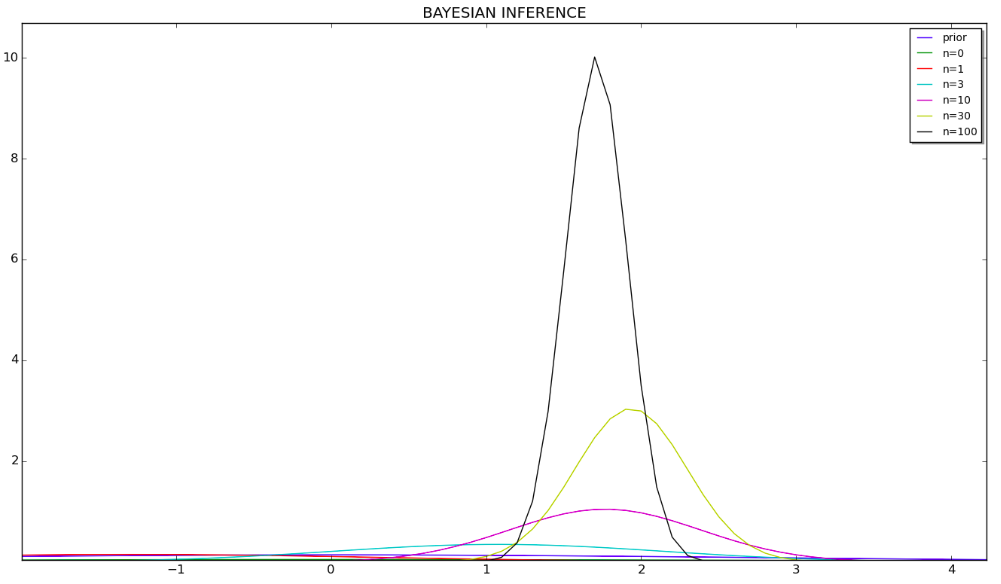
\includegraphics[width=1\textwidth, angle=0]{figure_1.png}
	   \caption{inference of \(\mathcal{N}(x|2,4)\), starting by \(\mathcal{N}(x|0,8)\)}
	   \label{fig2}
         \end{figure}
           




         
\end{document}




\begin{flushright}
  $\square$\\
\end{flushright}
